
\subsection*{1.10 Sets}
Set theory is a fundamental branch of mathematics that deals with collections of objects, called sets. These objects are called elements or members of the set. 

\textbf{Key Concepts:}
\begin{itemize}
    \item \textbf{Union of Sets:} The union of two sets $A$ and $B$, denoted by $A \cup B$, is the set of elements that are in $A$, in $B$, or in both.
    \[
    A \cup B = \{x \mid x \in A \text{ or } x \in B\}.
    \]

    \item \textbf{Intersection of Sets:} The intersection of two sets $A$ and $B$, denoted by $A \cap B$, is the set of elements that are in both $A$ and $B$.
    \[
    A \cap B = \{x \mid x \in A \text{ and } x \in B\}.
    \]

    \item \textbf{Complement of a Set:} The complement of a set $A$, denoted by $A'$, is the set of elements not in $A$ but in the universal set $U$.
    \[
    A' = \{x \in U \mid x \notin A\}.
    \]
    \item \textbf{Universal Set:} The universal set, denoted by $U$, is the set that contains all elements under consideration in a particular context. All subsets are defined within this universal set.

    \item \textbf{Cardinality of a Set:} The cardinality of a set $A$, denoted by $|A|$, is the number of elements in the set.

    \item \textbf{Venn Diagrams:} Venn diagrams are visual representations of sets and their relationships, such as union, intersection, and complement.


\end{itemize}

\begin{center}
    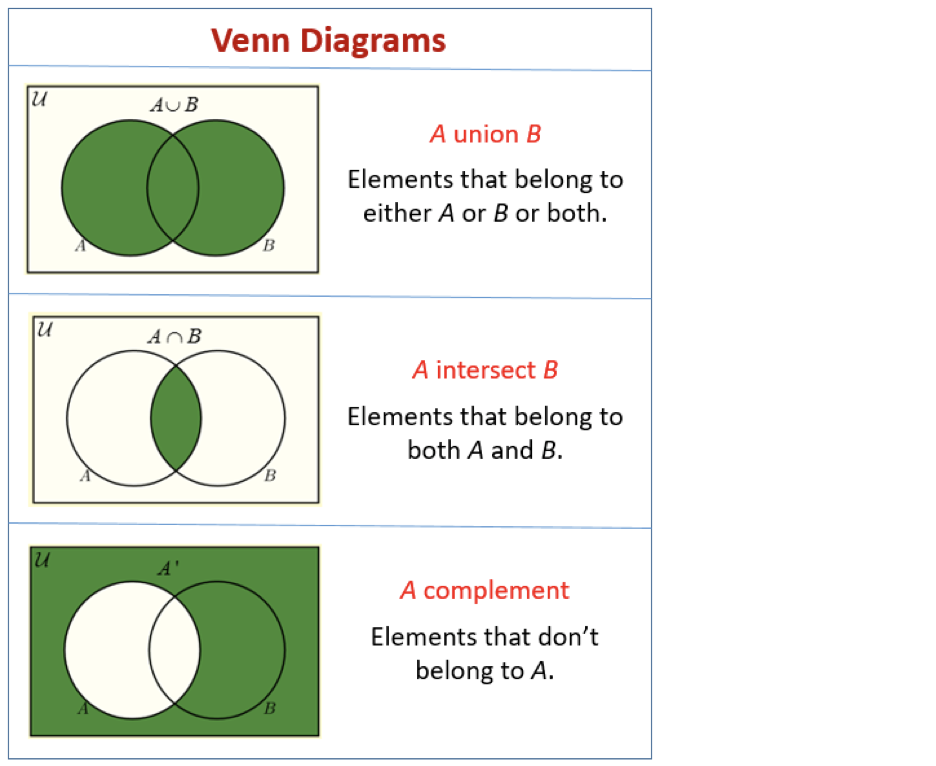
\includegraphics[width=0.7\textwidth]{1.1.png}
\end{center}



\begin{flushleft}
\textbf{Example 1: Union of Two Sets}

Given $A = \{1, 2, 3, 4\}$ and $B = \{3, 4, 5, 6\}$, find $A \cup B$.

\vspace{0.5cm}
\textbf{Solution:}
\vspace{0.5cm}

Step 1: Combine all unique elements of $A$ and $B$:
\[
A \cup B = \{1, 2, 3, 4, 5, 6\}.
\]

Therefore, $A \cup B = \{1, 2, 3, 4, 5, 6\}$.

\vspace{1cm}
\textbf{Example 2: Intersection of Two Sets}

Given $A = \{1, 2, 3, 4\}$ and $B = \{3, 4, 5, 6\}$, find $A \cap B$.

\vspace{0.5cm}
\textbf{Solution:}
\vspace{0.5cm}

Step 1: Identify the common elements in $A$ and $B$:
\[
A \cap B = \{3, 4\}.
\]

Therefore, $A \cap B = \{3, 4\}$.
\end{flushleft}

\begin{flushleft}
\textbf{Example 3: Complement of a Set}

Given $U = \{1, 2, 3, 4, 5, 6, 7\}$ and $A = \{2, 4, 6\}$, find $A'$.

\vspace{0.5cm}
\textbf{Solution:}
\vspace{0.5cm}

Step 1: List all elements in $U$ that are not in $A$:
\[
A' = \{1, 3, 5, 7\}.
\]

Therefore, $A' = \{1, 3, 5, 7\}$.
\end{flushleft}

\begin{flushleft}
\textbf{Example 4: Cardinality of Sets and Venn Diagram Application}

In a survey, 20 students like basketball, 15 like football, and 10 like both sports. How many students like at least one of the two sports?

\vspace{0.5cm}
\textbf{Solution:}
\vspace{0.5cm}

Step 1: Use the principle of inclusion-exclusion:
\[
|A \cup B| = |A| + |B| - |A \cap B|.
\]

Step 2: Substitute the values:
\[
|A \cup B| = 20 + 15 - 10 = 25.
\]

Therefore, 25 students like at least one of the two sports.
\end{flushleft}

